\documentclass[border=8pt]{standalone}
% Shared preamble for IronClaw thesis figures (standalone TikZ).
\renewcommand{\familydefault}{\sfdefault}
\usepackage{tikz}
\usetikzlibrary{arrows.meta,positioning,calc,fit,backgrounds,shapes.geometric,shapes.misc}

% IronClaw palette (matches slides.tex)
\definecolor{IronDark}{HTML}{1A2B3C}
\definecolor{IronBlue}{HTML}{2E86AB}
\definecolor{IronTeal}{HTML}{06A77D}
\definecolor{IronOrange}{HTML}{F18F01}
\definecolor{IronRed}{HTML}{C73E1D}
\definecolor{IronLight}{HTML}{F4F7F9}
\definecolor{IronGray}{HTML}{5D6D7E}

\tikzset{
  figtitle/.style={font=\large\bfseries\color{IronDark}, align=center},
  hostbox/.style={draw=IronBlue, rounded corners=5pt, fill=IronBlue!8,
                  line width=1pt, align=center, font=\small\color{white}},
  hostfill/.style={draw=IronBlue, rounded corners=4pt, fill=IronBlue,
                   line width=0.8pt, align=center, font=\small\color{white},
                   text width=3.1cm, minimum height=0.85cm},
  guestfill/.style={draw=IronOrange, rounded corners=4pt, fill=IronOrange!85,
                    line width=0.8pt, align=center, font=\small\color{white},
                    text width=3.1cm, minimum height=0.85cm},
  guestsoft/.style={draw=IronOrange, rounded corners=4pt, fill=IronOrange!25,
                    line width=0.8pt, align=center, font=\small\color{IronDark},
                    text width=3.1cm, minimum height=0.75cm},
  arrow/.style={-{Latex[length=2.6mm,width=2mm]}, line width=0.9pt, IronDark},
  biarrow/.style={{Latex[length=2.6mm,width=2mm]}-{Latex[length=2.6mm,width=2mm]},
                  line width=0.9pt, IronDark},
  note/.style={font=\footnotesize\color{IronGray}, align=center},
}

\begin{document}
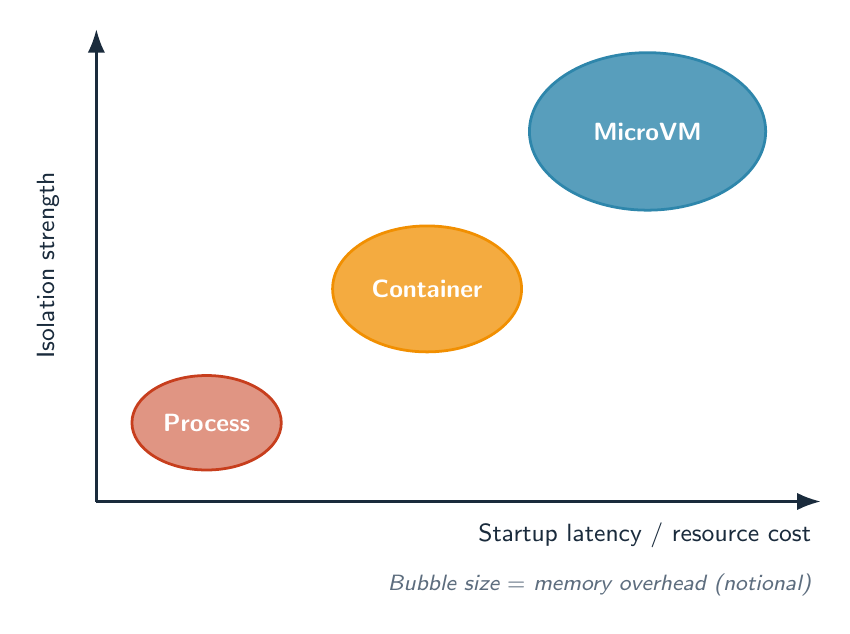
\begin{tikzpicture}
  \tikzset{
    bubble/.style={ellipse, line width=1pt, align=center, text=white,
                   font=\small\bfseries},
    axis/.style={-{Latex[length=3mm,width=2.2mm]}, line width=1pt, IronDark},
  }

  % axes
  \draw[axis] (0,0) -- (9.2,0);
  \draw[axis] (0,0) -- (0,6.0);
  \node[note, anchor=north east, font=\small\color{IronDark}] at (9.2,-0.15)
        {Startup latency / resource cost};
  \node[note, rotate=90, anchor=south, font=\small\color{IronDark}] at (-0.35,3.0)
        {Isolation strength};

  % bubbles: size grows with memory overhead
  \node[bubble, draw=IronRed,    fill=IronRed!55,    minimum width=1.7cm, minimum height=1.2cm]
        at (1.4,1.0) {Process};
  \node[bubble, draw=IronOrange, fill=IronOrange!75, minimum width=2.4cm, minimum height=1.6cm]
        at (4.2,2.7) {Container};
  \node[bubble, draw=IronBlue,   fill=IronBlue!80,   minimum width=3.0cm, minimum height=2.0cm]
        at (7.0,4.7) {MicroVM};

  \node[note, anchor=north east, font=\footnotesize\itshape\color{IronGray}] at (9.2,-0.8)
        {Bubble size \(=\) memory overhead (notional)};

\end{tikzpicture}
\end{document}
